\documentclass{article}
\usepackage{graphicx}
\usepackage{listings}
\usepackage[a4paper, total={6in, 8in}]{geometry}

\title{ComSci Project - MyTime}
\author{Max Stupple}
\date{}

\begin{document}
    
\maketitle{}

\part{Analysis}
\section{Overview of the problem}
Many students struggle to manage their time. The workload of A-levels alone is
enough to make it difficult to balance between small pieces that are due in
soon, and longer project that need a little bit of work here and there, let
alone extra-curricular activities and sports that take up more time after school
and on weekends. One solution is to manually plan how you will use all your free
time, but this has two drawbacks:
        
\begin{itemize}
\item Many people struggle to estimate how long a task will take them and hence
  struggle to allocate a reasonable amount of time to each task
\item This process takes time, a resource which has already been established to
  be finite and valuable
\end{itemize}

My stakeholder (henceforth referred to as SH) is a Year 12 Sixth Form student
studying Maths, Further Maths, Physics and Chemistry. He struggles to fit in all
his work around his various extra-curricular activities, so he needs an app that
will not only help him keep track of what he needs to do, but timetable when to
do each task and prioritise those which are most urgent. SH represents the needs
of my target user group.

\section{Limitations of current system}
To organise his tasks, SH currently uses the Apple Reminders app on his iPhone.
However, he finds this lacking for a number of reasons. Although the app helps
him keep track of the tasks he needs complete and when they are due, it does not
help him prioritise these tasks or inform him of the relationship between the
amount of time he needs to do those tasks and the amount of time he has before
they are due. He also doesn't find the app very engaging, as he lacks a sense of
accomplishment after completing a task and ticking it off his list. Furthermore,
the app only provides the ability to sync between Apple devices, which he finds
limiting as he cannot access his tasks on his Windows computer. SH also finds
the light theme of the app abhorrent, and desires a solution with a darker, more
attractive colour scheme.

\section{Initial ideas}
This initial feature list will help me research existing software which may
partially solve the problem. It will also give an idea of how complex the final
solution will be.

To satisfy the needs of SH, I anticipate a solution will need to fulfil the
following functions:

\begin{itemize}
\item Keep a list of the users tasks which contain a description of the task, a
  due date and time estimate
\item Schedule tasks in user's free time according to a calendar and school/work
  schedule
\item Record and track the actual time taken to complete a task, including
  breaks
\item Provide feedback on the accuracy of the user's time estimates and
  productivity levels
\item Adapt to the user's preference in terms of length of work sessions
\item Display these tasks to the user is an organised manner using a Graphical
  User Interface
\end{itemize}

The program will be created as a web app using the Django web framework. The
reason for creating it as a web app is so that it is available as widely as
possible, as it will be possible to access it on any device with a modern web
browser. Django will allow me to deploy my solution in a modern and efficient
way, so that I can focus on the underlying data structures, while Django mostly
handles the interface. The data structures will also be implemented using Python
in an object-oriented way, which I think is sensible and are tools I'm familiar
with working with.

\section{User group}
My target users are students, in particular Sixth Form and University. As the
program is targeted at individuals who struggle to manage their time and avoid
procrastination, the program will need to be engaging and provide incentives for
the user to complete tasks early rather than delaying them. Thus the user will
avoid situations in which they find themselves with insufficient time to
complete all their tasks before they are due.

The UI must also be simple and intuitive to use: there's no point in using an
app to organise your time if you waste more time trying to get the app to work
than doing the work you need to do.

\section{Computational methods}
This problem lends itself to a computational solution in particular due to the
need for automation and interactivity to ensure engagement. One potential
non-computational solution could be a physical calendar or to-do list, however
this would not be able to provide the features required by my client. Such a
solution could not automatically allocate time for the user to complete their
tasks in, and could not remind the user of their tasks - it would require the
user to check and plan the time for themselves.

\subsection{Abstraction}
Data will be stored with an object-oriented approach. Tasks, events, routine
events, and allocated time slots will all be objects with appropriate
relationships so that the data can be viewed from a number of perspectives.

\subsection{Reusability}
There are a number of functions which my program will need to perform where it
wouldn't make sense to write them myself from scratch, so I will use libraries
that have already solved the problem. I will need to be able to get the current
date and time, to associate with each task, and a SQL database to store my data
in.

\subsection{Visualisation}
My program will need to be able to present data to the user in a way that is
visually appealing and easy to understand. For example, data about the number of
tasks completed can be presented on a histogram.

\subsection{Concurrency}
The program will need to be able to perform certain tasks in the background
without interrupting the user, for example allocating time slots to tasks and
analysing data to create graphs and provide feedback to the user.

\subsection{Data Mining}
Albeit on a small scale, my program will use the concept of data mining to
analyse trends in the user's completion of tasks, such as how much time they
spend and how accurate their time estimates are, in order to give feedback and
help the user improve their efficiency.

\subsection{Logic}
The program will need to be able to intelligently allocate time slots to tasks
based on the user's schedule and the time needed to complete the task. It will
also need to be able to adapt the user's habits and preferences regarding their
work schedule.

\section{Research}
I identified a number of candidates for solutions to SH's problem. The candidate
programs are:

\begin{itemize}
\item Forest
\item Evernote
\item Todoist
\item Remember the Milk
\item Ike
\item Google Keep
\item Trello
\end{itemize}

\begin{figure}[h!]
  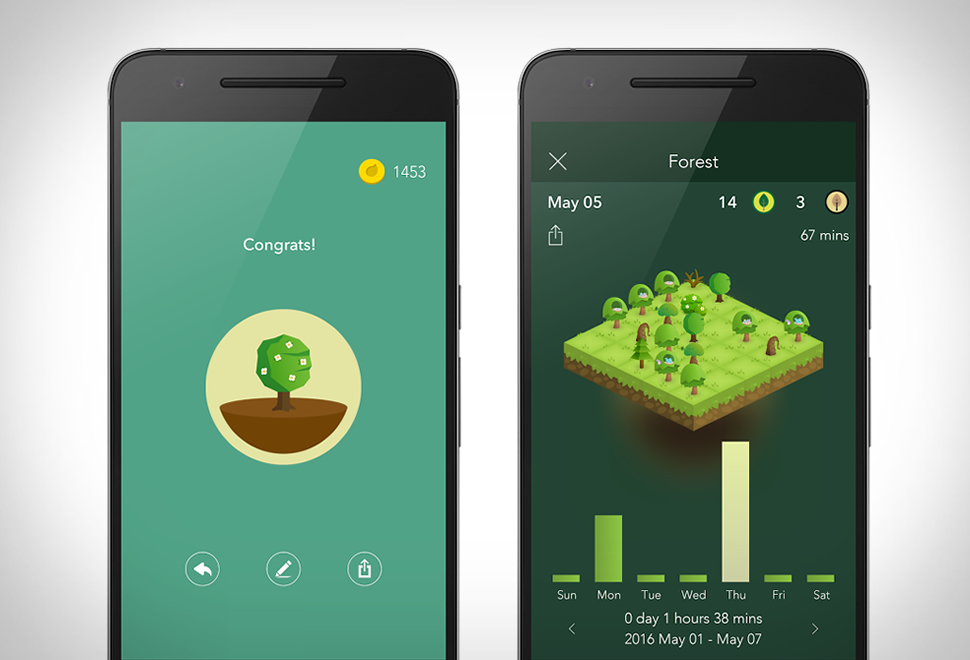
\includegraphics[width=\linewidth]{Images/forest.jpg}
  \caption{Forest}
  \label{fig:forest1}
\end{figure}

Forest is the only candidate dedicated to helping the user focus on their tasks
and get stuff done as quickly as possible by avoiding distractions. It's primary
feature is an animated forest which grows as you work, but dies if you leave the
app. This encourages the user to avoid 'quickly' having a look at Facebook,
sending a text or otherwise breaking their workflow. Forest shows you how much
time you spent each day growing your forest, so you can see which days you were
most productive on. The primary drawback of Forest is that it lacks any means of
tracking tasks from within the app. In my view this is significantly problematic
as the app which is going to help you focus the most is one which never needs
you to leave while working. Integrated task management is an
absolute must for my solution.

\begin{figure}[h!]
  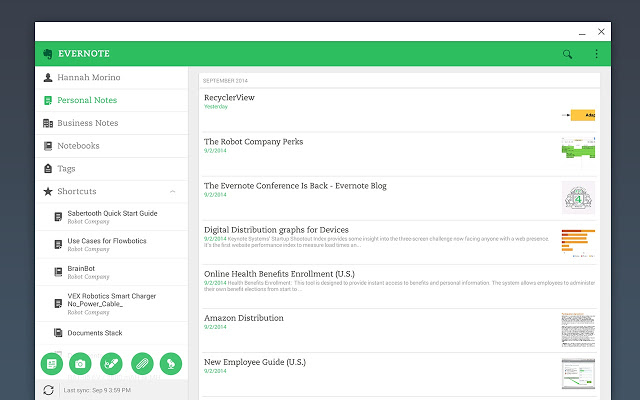
\includegraphics[width=\linewidth]{Images/evernote.jpg}
  \caption{Evernote}
  \label{fig:evernote1}
\end{figure}

Evernote is primarily focused on note-taking, organisation and task-management.
The power of it's note-taking is remarkable, and can include voice memos,
handwritten notes and embedded web pages. However, most of these features are
superfluous for my product, and would needlessly add complexity.

\begin{figure}[h!]
  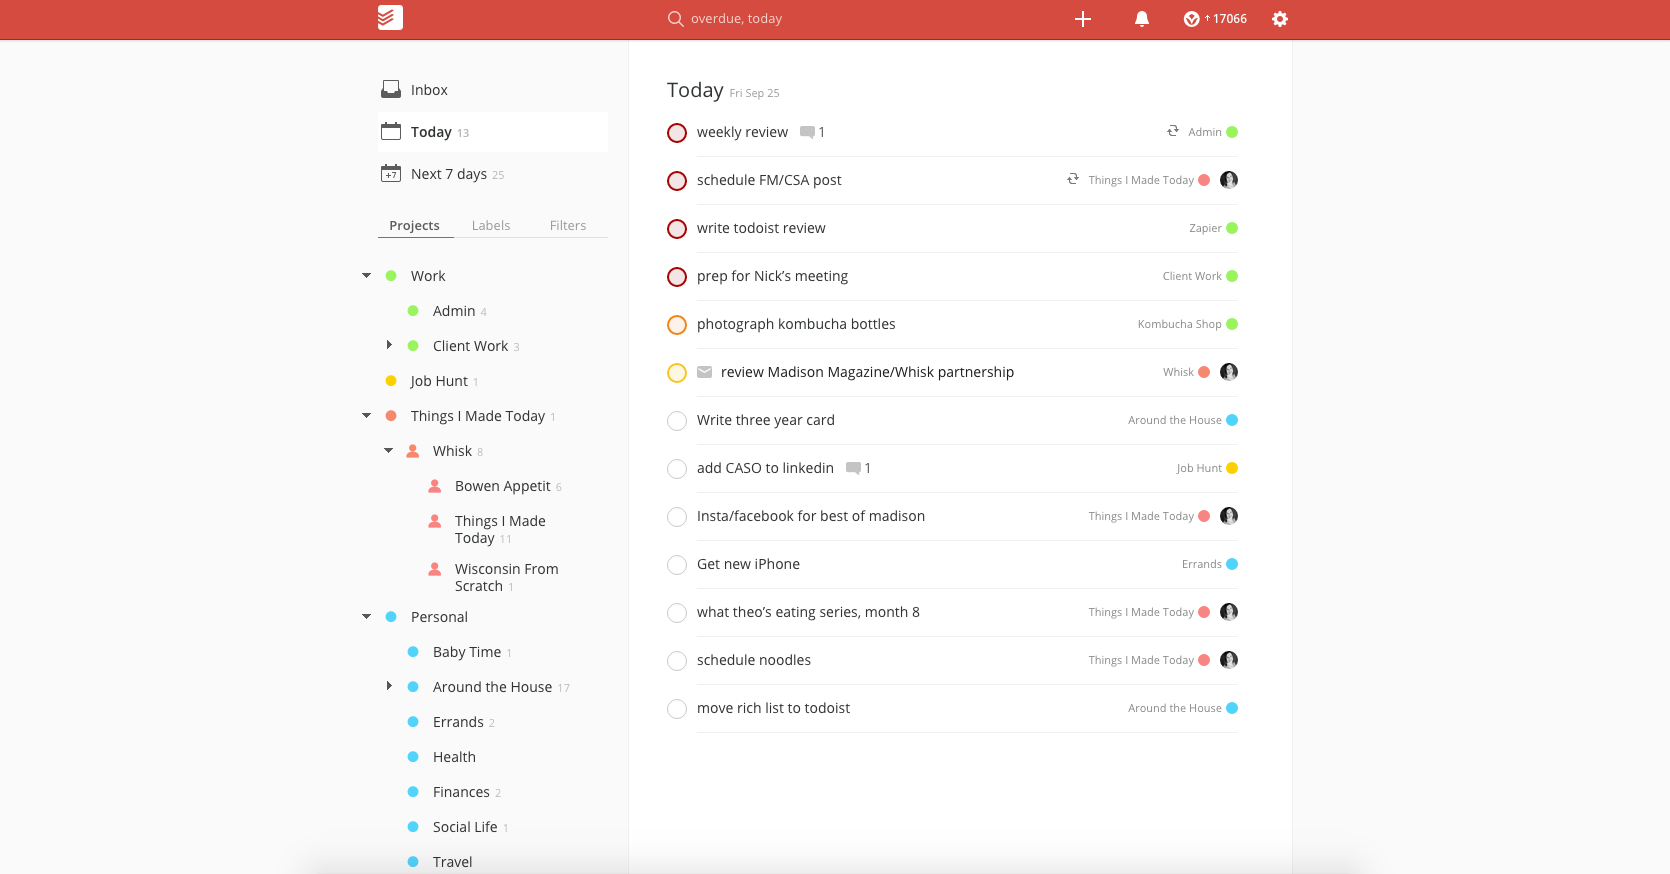
\includegraphics[width=\linewidth]{Images/todoist.png}
  \caption{Todoist}
  \label{fig:todoist1}
\end{figure}

Todoist is the only of these apps which is laser-focused on to-dos. One of its
prominent features is the ability to write tasks in natural language, which it
then understands when they are due, if they are recurring etc. This is beyond
the scope of my product, however I am interested in the tools they have for
tracking your productivity. Todoist can display graphs of total number of tasks
done per day/week, the distribution between different types of tasks e.g.
whether you did more tasks tagged with ``Study'' or ``Chores''. I definitely
want to have similar visualisations of how productive the user is being.

\begin{figure}[h!]
  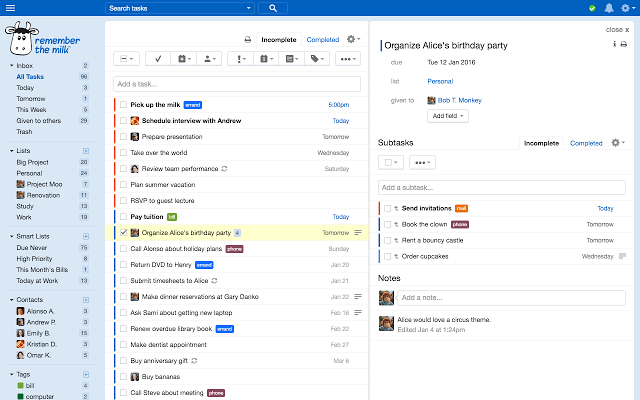
\includegraphics[width=\linewidth]{Images/remember-the-milk.png}
  \caption{Remember The Milk}
  \label{fig:rtm1}
\end{figure}

Similar to Todoist, Remember the Milk has a lot of advanced tools for
intelligently adding, sorting and searching through tasks. However I'm
particularly interested in the ability to divide tasks into sub-tasks. I
personally have used to-do apps with such a feature and have found it rather
useful, so I'll be interested to get my stakeholder's opinion on this
feature specifically when I talk to them.

\begin{figure}[h!]
  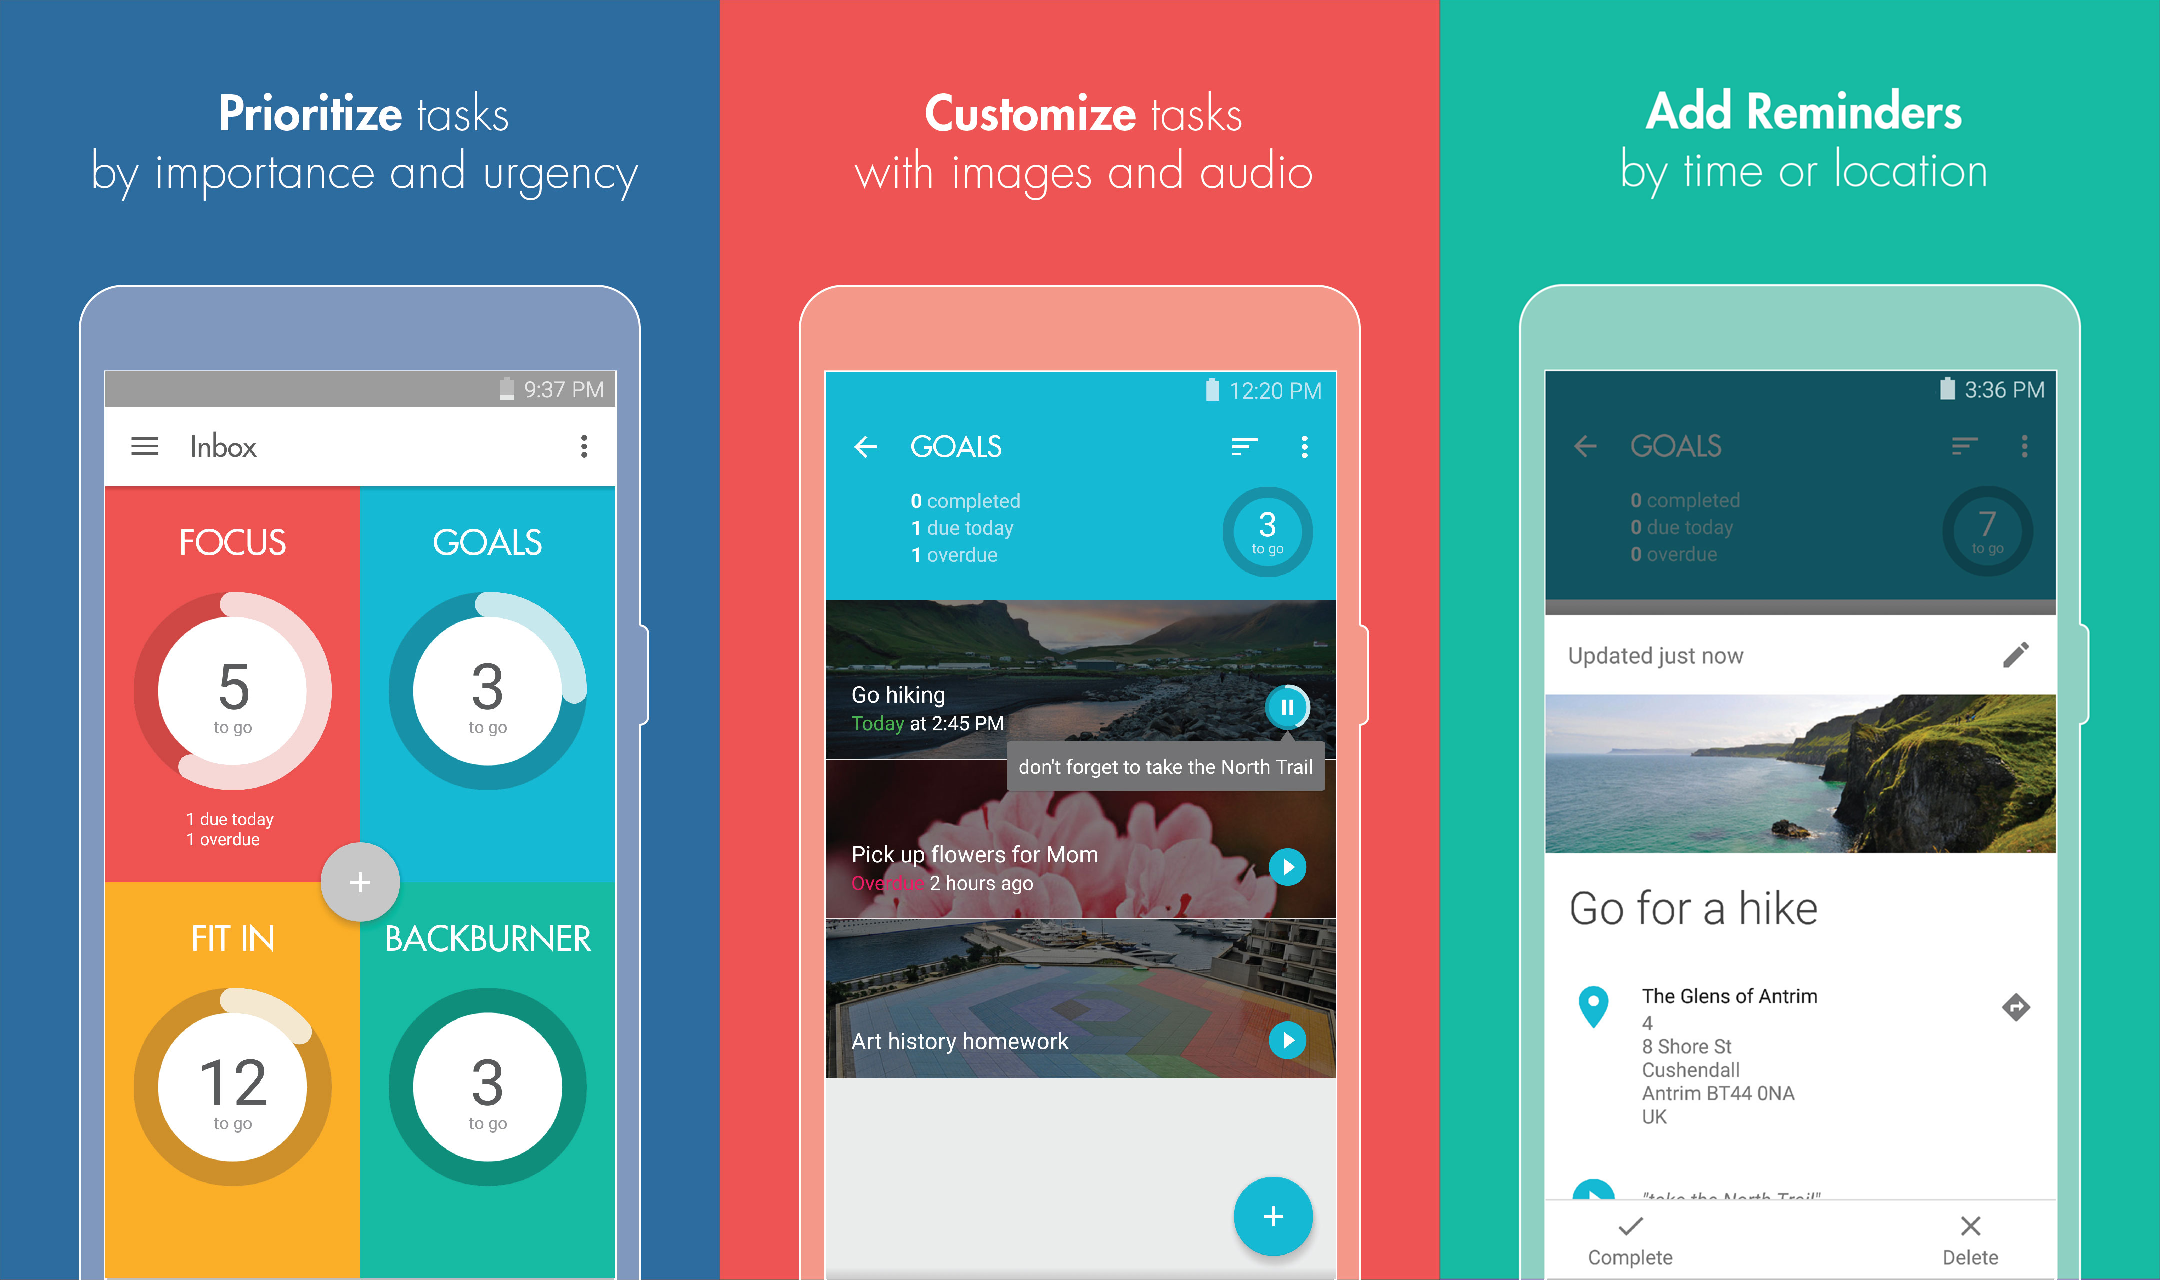
\includegraphics[width=\linewidth]{Images/ike.png}
  \caption{Ike}
  \label{fig:ike1}
\end{figure}

Ike is in fact the to-do app which I currently use. I can't say that I'm
entirely satisfied with it, but I like the system of organising tasks into
``Urgent and Important'', ``Urgent but not Important'', ``Important but not
Urgent'' and ``Neither Urgent nor Important''. I think this is a useful system
and could perhaps be preset in my product, but I find it limiting that Ike
forces you to organise by those categories. I definitely want my product to
allow the user to organise their tasks into whatever folders and sub-folders
they please. I think any limitation on how the tasks are organised will always
be counterproductive in some degree to some users.

\begin{figure}[h!]
  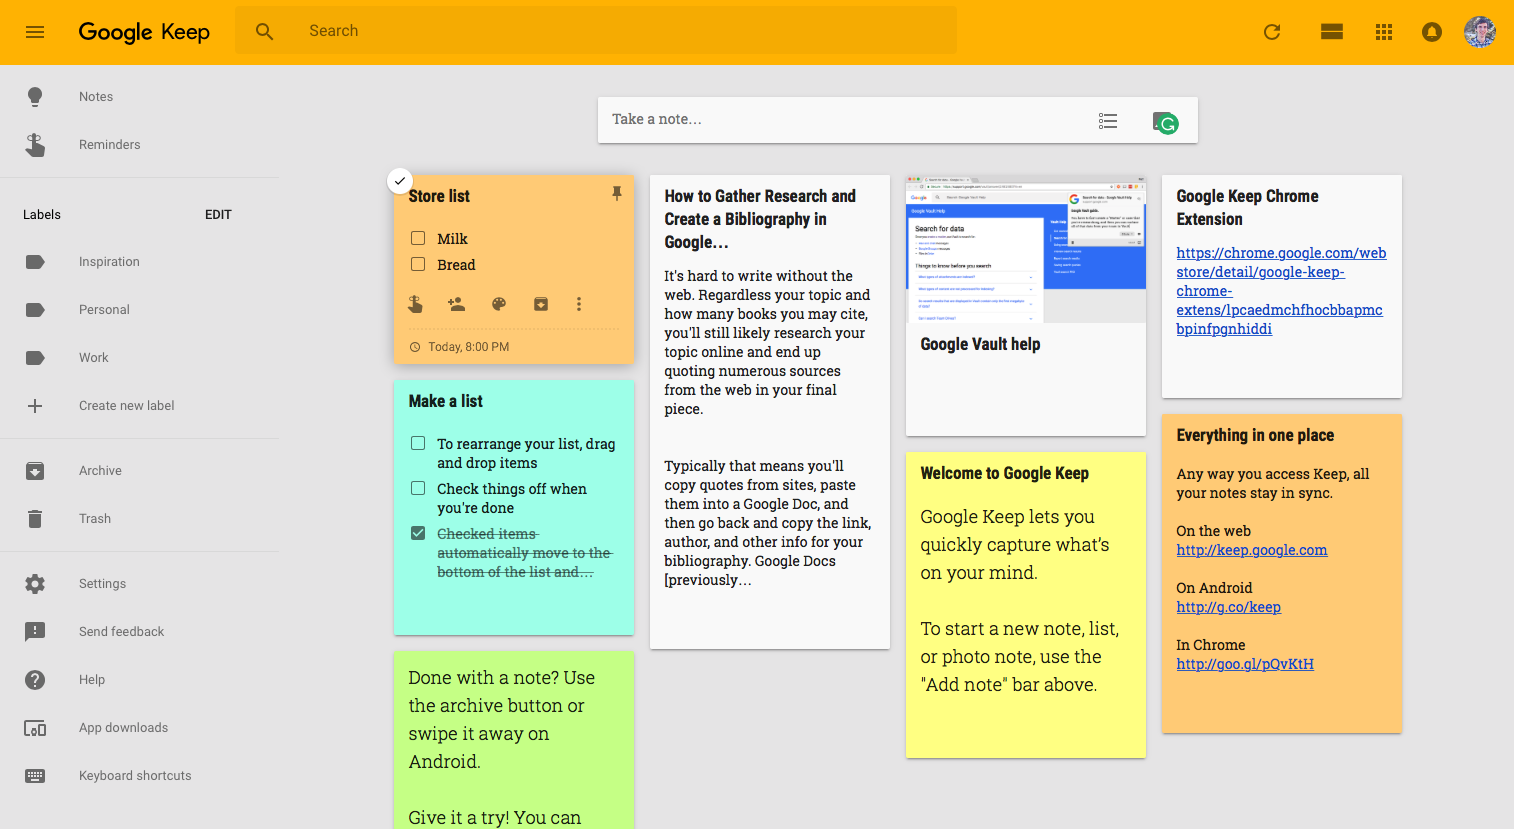
\includegraphics[width=\linewidth]{Images/keep.png}
  \caption{Google Keep}
  \label{fig:keep1}
\end{figure}

Keep is quite a good, basic to-do app. Keep's main interesting feature is its
integration with the rest of Google's ecosystem, however this isn't really
something that my project is too concerned with. I'm also not a fan of Keep's
visual metaphor of tasks being ``cards'' on the screen - a common visual
metaphor in Google's design language. I think this creates confusion as there is
not simply a vertical list. I also dislike that you need to create different
types of tasks for simple text, lists, voice memos etc.

\begin{figure}[h!]
  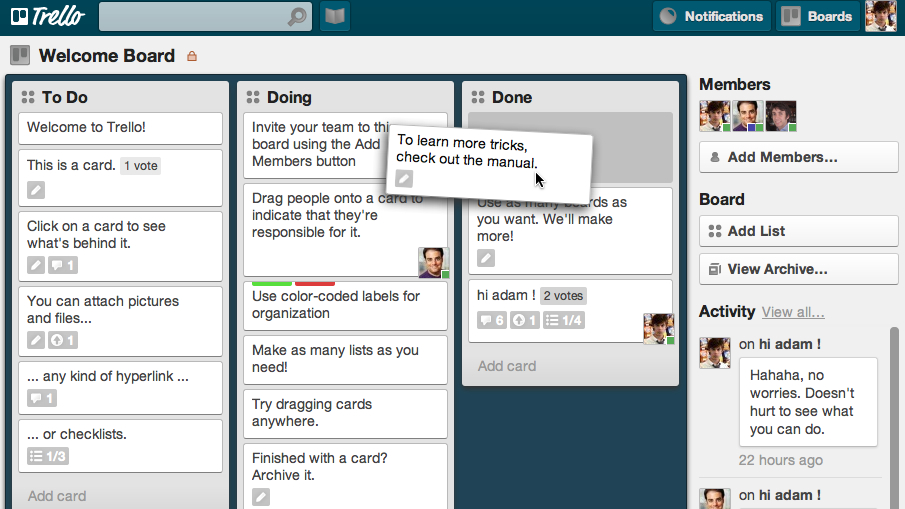
\includegraphics[width=\linewidth]{Images/trello.jpg}
  \caption{Trello}
  \label{fig:trello1}
\end{figure}

Trello is more focused on managing multi-person projects than an individual's
todo list. It's most prominent feature is the ability to work collaboratively on
creating tasks, marking them complete, adding comments and so on. However I
think this sort of feature is beyond the scope of my solution. However I do like
that each ``card'' can - unlike Keep - have text, checklists, and attachments. I
think it will be useful for my users to be able to attach a reasonable amount of
information to their tasks.

I think these programs all offer partial solutions to the problem, but none of
them offer a solution to the exact problem SH has described. Forest is excellent
for helping you focus on a task, but can't keep track of your to-dos. Todoist
offers excellent functionality for keeping track of and organising your tasks,
but doesn't do anything with regard to helping you timetable everything that you
need to do. Keep is better in this regard as it integrates with GCal to display
tasks in your calendar, but can't allocate them those time slots automatically.
Ike has a very appealing UI and a good system for organising into four
overarching categories, but you can't create your own categories like Todoist.
Remember the Milk is probably the most intelligent of the programs, with a
``Smart Add'' feature that makes adding tasks very simple, and a powerful search
for filtering through your tasks, in addition to integrating with a number of
other services such as email and social media for reminders, and cloud storage
services for adding attachments to tasks, however this is probably beyond the
scope of the problem I'm trying to solve. Evernote is in my opinion the least
effective of these programs, as it is mainly focused on note taking, with
reminders as a side-feature. Trello offers the most features oriented towards
time management and prioritising tasks, but is more focused around team
collaboration on big projects than individual to-do management.

I showed the candidates to SH to get his opinion and he gave me the following
comments:

\begin{description}
\item Forest: ``This is my favourite. The UI is excellent and the metaphor of
  growing trees is very appealing. Out of all the programs this does the best
  job of helping me manage my time, however tt's unfortunate that is doesn't
  include integrated task management. I like that you can see your past progress
  as this is very motivational, and it stops the timer if you leave the app,
  which helps you avoid idly switching to Facebook or Twitter for a 'quick
  check'.''
\item Evernote: ``Good for note taking, but that's not really what I'm looking
  for. It has too many extraneous features, which are unnecessary and make it
  feel bloated - I want a more streamlined experience. I also dislike the
  subscription model.''
\item Todoist: ``Great for managing tasks, with graphs and data to track your
  statistics. I love the categorisation and colour coding for different tasks,
  and being able to give them different levels of priority. I also like that you
  can export your tasks to your calendar. The lack of a dark mode harms the
  UX.''
\item Remember the Milk: ``There's too much task segregation which makes the UI
  confusing. It also has a weird notes system. Not a fan.''
\item Ike: ``The idea behind it is admirable, but ultimately the categories feel
  a bit arbitrary, and that's made worse by the lack of an 'all tasks' view. The
  UI is very clean however, and the animations are really nice.''
\item Keep: ``It's good for lists, but otherwise nothing special.''
\item Trello: ``Good for project development, but not well-suited to personal
  task management.''
\end{description}

He also commented in general that he liked the ability to sync tasks between
devices, and a feature which he wanted but none of the programs offered was the
ability to have ``subtasks'' nestled inside other tasks.

From this I have assembled the following list of features which my program will
need:

\begin{itemize}
\item Main view displays all uncompleted tasks and recently completed but
  not-deleted tasks
\item Archive containing completed tasks, and allows tasks to be un-marked as
  complete
\item Tasks grouped in categories, can be colour coded
\item Tasks can be filtered by category
\item Ordered by time needed or due date
\item Tasks can be marked as done or deleted
\item New tasks can be added, with a brief title, optional additional notes, an
  estimate of time needed and a due date
\item Graphs showing number of tasks completed, amount of time taken, and
  whether tasks were completed on time
\item Show upcoming tasks in their automatically allocated time slots
\item User can enter the schedule and other commitments that the program will
  schedule tasks around
\item The program will give a warning if there is not enough free time to
  complete a given task before it's due date
\item Current task displayed at top of screen
\item Time spent working and time to next break
\item Buttons to manually pause timer and take a break or mark task as done
\item Graphic showing a town/city building up over time as you work
\end{itemize}

I showed this list to SH, and he added that tasks should be given a priority
level, so that high priority tasks can be scheduled before low priority ones. He
also elaborated on the city-building mechanic, resulting in the following:

\begin{itemize}
\item The city builds over time as you work
\item Taking a break which has been allocated by the app simply pauses
  development
\item Taking an unallocated break sets the development back - perhaps there is a
  level system and you can be set back one or two levels
\item If you quit a task before you finished - and taking an excessively long
  break automatically quits - the city is destroyed
\item If you take too long to complete a task, development is slowed down
\item When you finish a task, you can either stop, which doesn't destroy your
  city but it degrades over time, or go straight to the next task, in which case
  progress continues
\item If you finish a task early and go straight on to another task, your city
  gets a boost
\end{itemize}

SH said he ``agrees with all of this'' and called it ``good design''. He also
emphasised his desire to access his tasks across different devices. I have
concluded that the best way to facilitate this would be to build the program as
a web app. This is the easiest way to make it available cross-platform, as it
should be accessible on any device with a modern web browser.

SH also suggested that there were psychological benefits to offering the user a
choice in what task they do. Studies have shown that individuals are more
motivated to complete a task which they have chosen to do from a set of options,
rather than only one. Therefore I will endeavour to implement a system which,
rather than forcing, or heavily encouraging, the user to complete one particular
task in a certain time slot, will instead give them the option to choose between
tasks with similar levels of priority.

\section{System requirements}
As the program will be web-based, it will require a system capable of running a
modern internet browser, such as Firefox. The system requirements for Firefox
66.0 are as follows:

\subsection*{Windows}\label{windows}

\subsubsection*{Operating Systems (32-bit and
  64-bit)}\label{operating-systems-32-bit-and-64-bit}

\begin{itemize}
\item Windows 7
\item Windows 8
\item Windows 10
\end{itemize}

\subsubsection*{Recommended Hardware}\label{recommended-hardware}

\begin{itemize}
\item Pentium 4 or newer processor that supports SSE2
\item 512MB of RAM / 2GB of RAM for the 64-bit version
\item 200MB of hard drive space
\end{itemize}

\subsection*{Mac}\label{mac}

\subsubsection*{Operating Systems}\label{operating-systems}

\begin{itemize}
\item macOS 10.9
\item macOS 10.10
\item macOS 10.11
\item macOS 10.12
\item macOS 10.13
\item macOS 10.14
\end{itemize}

\subsubsection*{Recommended Hardware}\label{recommended-hardware_1}

\begin{itemize}
\item Macintosh computer with an Intel x86 processor
\item 512 MB of RAM
\item 200 MB hard drive space
\end{itemize}

\subsection*{GNU/Linux}\label{gnulinux}

\subsubsection*{Software Requirements}\label{software-requirements}

\emph{Please note that GNU/Linux distributors may provide packages for your
  distribution which have different requirements.}

\begin{itemize}
\item Firefox will not run at all without the following libraries or packages:

  \begin{itemize}
  \item GTK+ 3.4 or higher
  \item GLib 2.22 or higher
  \item Pango 1.22 or higher
  \item X.Org 1.0 or higher (1.7 or higher is recommended)
  \item libstdc++ 4.6.1 or higher
  \end{itemize}
\item For optimal functionality, we recommend the following libraries or
  packages:

  \begin{itemize}
  \item NetworkManager 0.7 or higher \index{\item}\index{\item}\item DBus 1.0 or
    higher
  \item GNOME 2.16 or higher
  \item PulseAudio
  \end{itemize}
\end{itemize}

Any system which meets these requirements will be able to run the program.

\section{Success Criteria}

\subsection{General objectives}
To create a program which stores tasks and arranges them around the user's
schedule. The program should engage the user through the use of a game-like
progression system and help the user complete their tasks in a timely manner
through the use of reminders.

\subsection{Specific objectives}
The program should:

\begin{itemize}
\item Store a list of the user's tasks
\item Store the due date, priority, expected time needed, and other information
  about each task
\item Add and remove tasks from the list
\item Allow the user to group tasks into categories of their choosing, and
  colour code categories
\item Record the successful completion of each task, time taken, and number of
  breaks taken and display this information to the user in a useful manner
\item Schedule time for the user to complete their tasks, according to the
  user's schedule, task due date, task priority, and the user's preferences
\item Display the tasks in their allocated time slots in a calendar view, and
  allow the user to manually alter time allocations
\item Have a focus mode, which helps the user concentrate on the task at hand,
  and incentivise the user to complete the task in a timely manner without
  procrastination using game-like aspects
\item Be available on multiple platforms and devices
\item Sync tasks between devices
\item Remind the user of upcoming tasks
\end{itemize}


\part{Design}
\section{Breaking down the problem}
The first step to solving the problem is to decompose it into modules,
which will comprise the overall solution.
This is a higher-level description than the product specification,
but low enough that each component is a manageable individual problem.
I have identified the key functions that my solution will need to perform as:
\begin{itemize}
\item Basic calendaring:\\
  My solution needs to keep track of the user's regular commitments,
  and particular events,
  so that tasks can be scheduled around them.
\item Task management:\\
  The user should be able to add tasks,
  mark them as done,
  and delete them.
  These tasks should be able to hold a reasonable amount of information,
  but in particular a due date and time estimate will be essential to the scheduler.
\item Track time spent on tasks:\\
  The user should be able to log they are working on a task,
  and for how long,
  so that they can see overall statistics,
  on the accuracy of their time estimates,
  and on how good they are at sticking to their schedule.
\item Calculate and display statistics:\\
  The aforementioned statistics should be presented to the user in a helpful way.
\item Scheduling the user's tasks:\\
  The program will need to allocate time for each of the user's tasks,
  according to their priority,
  due date,
  and time estimate.
  It will also need to take into account the user's other commitments.
\end{itemize}

\begin{figure}[h]
  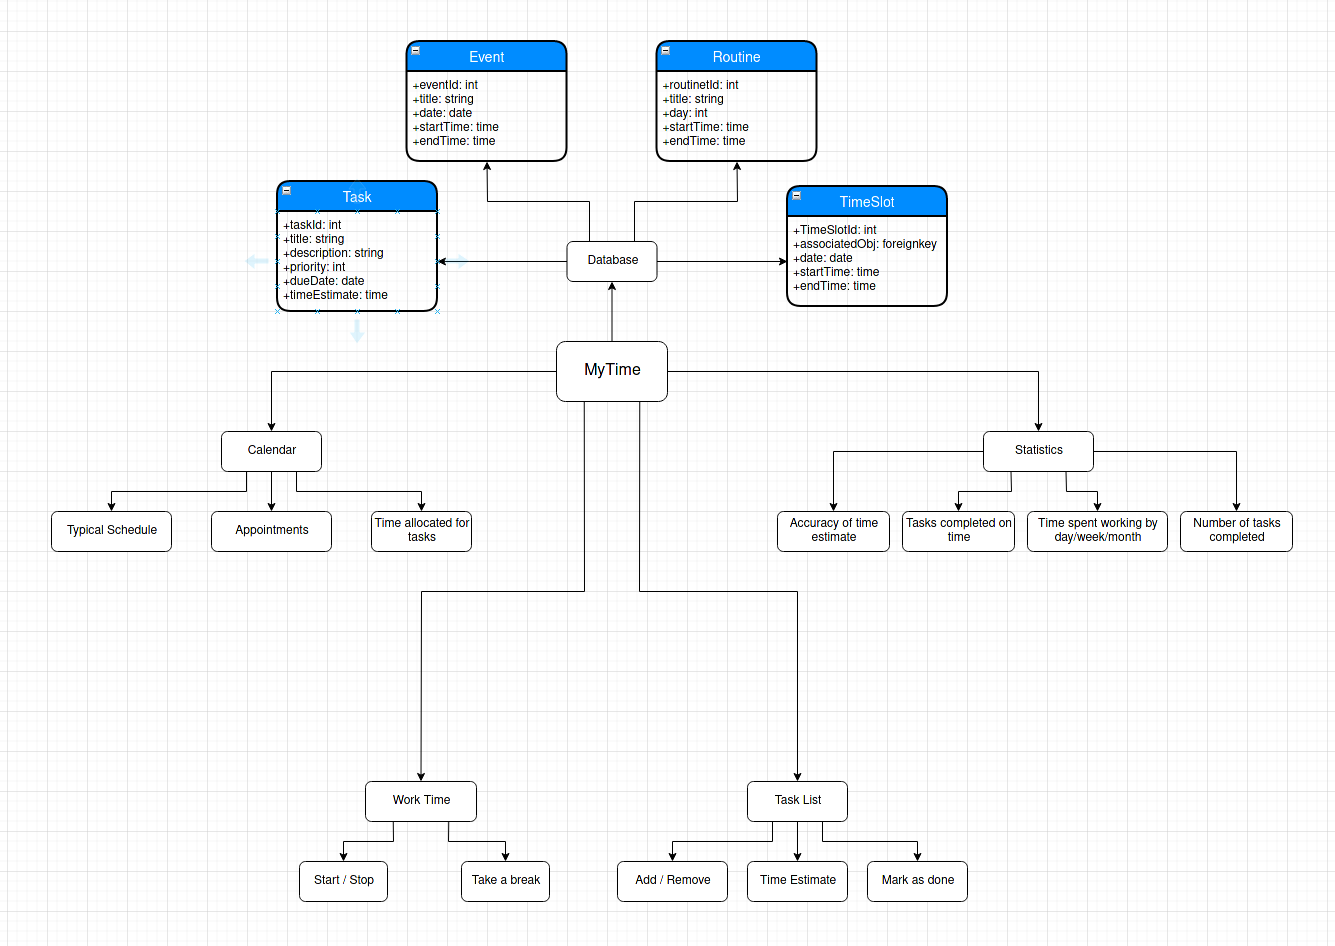
\includegraphics[width=\linewidth]{Images/TDD.png}
  \caption{Combination of top-down design analysis and class diagrams}
  \label{fig:TDD1}
\end{figure}

\subsubsection{Explanation of design}
The solution naturally breaks down into four parts:
a task manager,
a basic calendar,
a tracker for time spent working,
and a statistics viewer.
The relevant data that each component will need to use is also quite obvious:
the task manager, time tracker and statistics tracker will only be concerned with tasks,
whereas the calendar will additionally need the user's routine, daily commitments,
and any particular events that tasks will need to be scheduled around.

The data, then, will consist of four types.
Tasks will have a title and description,
so the user can record a reasonable amount of information alongside them,
and a due date, time estimate and priority level,
so that they can be scheduled.
Events and routines are similar,
however differ in that whereas events have a concrete date,
routines have a weekday on which they reoccur.
Both have a title, start and end time.
The TimeSlot exists for the purposes of unifying data into a single type for the purposes of scheduling.
They have a data, start and end time as expected,
and additionally an associated object,
being the task, event or routine which occupies that slice of time.
It might be possible to remove the need for this additional data structure,
by instead converting tasks and routines into events for the purpose of scheduling,
however it makes sense to logically distinguish between tasks, events and routines,
which represent user intentions -
what the user wants to do with their time -
and time slots,
which represent a concrete allocation of time to be used for a specific purpose.
Of course events and routines are already concrete,
as the program will never override them since this would not be helpful for the user,
but it is a nice logical separation to make in the database,
which wouldn't be possible if I instead used the approach of converting everything into events for scheduling.
Furthermore it would bloat event records with fields that would often go unused,
depending on whether it was a regular event or a wrapper around a task or routine,
so it seems more elegant to have a separate class for time slots.

\subsection{UI Design}
It seems sensible for this sort of product that I would want a navigation bar,
shared by every screen,
with the content below.

I will have the following views:
\begin{itemize}
\item Task list:\\
  A screen where the user can create, view and manage their tasks
\item Calendar:\\
  A screen where the user can create, view and manage upcoming events
\item Schedule:\\
  A screen showing the users tasks scheduled in around their events for today
\item Task/event/routine detail:\\
  A screen where the user can look at and individual task, event or routine,
  and perform relevant actions such as marking as done/todo,
  editing or deleting them
\item Task/event/routine creator:\\
  A form to create new tasks, events or routines
\item Task/event/routine editor:\\
  A form to edit existing tasks, events or routines
\item Work time:\\
  A screen where the user can enter a ``work session'' which records the time they spend working
\item Work review:\\
  A screen displaying statistics about the time the user has spent working
\end{itemize}

I think it will be simplest and most intuitive to have a navigation bar,
at the top of the screen,
allowing the user to quickly jump between the five main views -
task list, calendar, schedule, work time and work review -
and have individual tasks and events accessible from those views.
It might also be helpful to have a quick button to add a new task/event/routine.

\part{Development}
\section{Stage 0: Learning Django}
I haven't used Django before,
so before I really get started on building my project I need to learn the basics.
Fortunately, Django have a very helpful and comprehensive tutorial,
as well as detailed and easy to navigate documentation.

I decided first of all to run through the standard tutorial,
which involves building a website for hosting various polls.
In fact, this turned out to be incredibly useful because the structure of this website bears a number of similarities to my project:
the main screen is a list of various polls,
which you can then click on to view more information about and interact with.
I will similarly need to have screens with lists of tasks and events,
which you can then view in more detail and edit or mark as done etc.

\subsection{Models and Views}
I understand that Django is oriented around two primary data structures:
models and views.
Models are classes in Python,
but they are also the tables in the database,
with the attributes of the class corresponding to the fields,
and instances to specific records.
Being objects, they can also have methods.
These don't correspond to anything in the database,
but are useful for manipulating data.
I imagine, for example, that I will want my Task model to have a mark as done method when I come to implement it.

Views, on the other hand, correspond to the frontend.
They outline what data will be viewed on each page,
and also vaguely specify the appearance of the page,
although this is controlled more precisely in HTML ``templates''.

Here is an example model from the polls tutorial:
\begin{lstlisting}[language=Python]
class Question(models.Model):
    question_text = models.CharField(max_length=200)
    pub_date = models.DateTimeField('date published')

    def __str__(self):
        return self.question_text

    def was_published_recently(self):
        return self.pub_date >= timezone.now() - datetime.timedelta(days=1)
\end{lstlisting}

In the database,
this corresponds to a table called ``Question'',
with fields ``question\_text'' and ``pub\_date'',
holding text and datetimes respectively.

Here's a screenshot of the that table:

\begin{figure}[h!]
  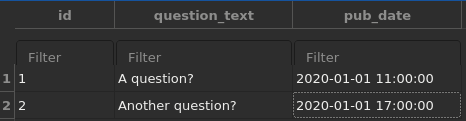
\includegraphics[width=\linewidth]{Images/question_table.png}
  \caption{Database table ``Question''}
  \label{fig:database1}
\end{figure}

As you can see,
Django also automatically includes a primary key ``id'' field with each table.

The model also has the methods ``\_\_str\_\_'' and ``was\_published\_recently'',
which are not seen in the database,
but rather make it quicker and easier to use the data within Python.

Here is an example view from the polls tutorial:
\begin{lstlisting}[language=Python]
class IndexView(generic.ListView):
    template_name = 'polls/index.html'
    context_object_name = 'latest_question_list'

    def get_queryset(self):
        # Return the last five published questions.
        return Question.objects.order_by('-pub_date')[:5]
\end{lstlisting}

The queryset for this view is the five most recently published objects in the Question table.
It then uses the template located at ``templates/polls/index.html'' -
the root folder ``templates'' is implicit.
Here is that template:
\begin{lstlisting}[language=HTML]

   <ul>
       
       <li><a href="/polls/{{ question.id }}/">{{ question.question_text }}</a></li>
       
   </ul>

   <p>No polls are available.</p>

\end{lstlisting}

Unless ``latest\_question\_list'' is empty,
this will output a list of the five most recent questions,
showing their names and linking to that question's page.
The URLs are defined in the aptly names urls.py.

\section{Stage 1: Tasks}


\end{document}

% LocalWords:  MyTime Evernote Trello Todoist subtasks TimeSlot
